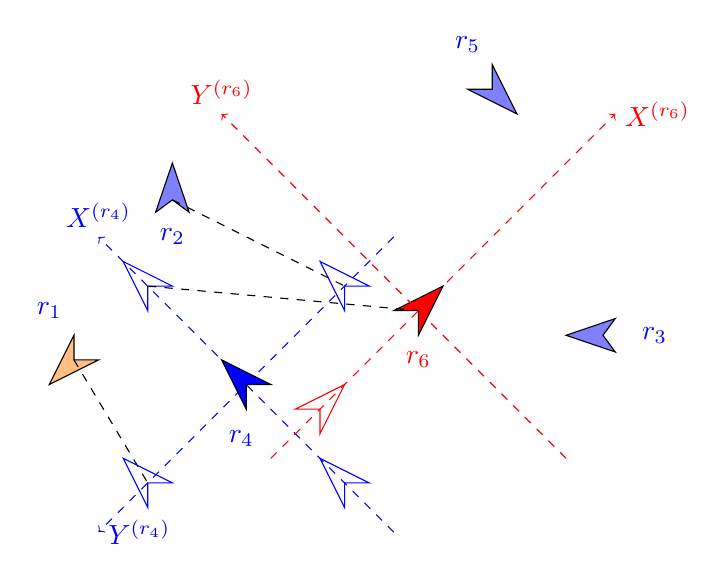
\begin{tikzpicture}[scale=1.25]
    \draw[fill=red] (3,3) -- (2.75,3) -- (3.25,3.25) -- (3,2.75)        -- cycle;
    \node[color=red] at (3, 2.5) {$r_6$};
    %\draw[thick, ->] (-1,0) -- (6,0) node[right] {X};
    %\draw[thick, ->] (0,-1) -- (0,6) node[above] {Y};
    % draw grids
    %\draw[color=gray, help lines, line width=.05pt] (-1,1)  grid[xstep=.5cm, ystep=.5cm] (6,6);
    % center of rc : 0.5, 4.125
    \def\Cx{0.5}
    \def\Cy{4.125}
    \def\d{1.5}
    \def\dd{1}
    \coordinate (C) at (\Cx, \Cy);
    \def\Ex{1.25}
    \def\Ey{2.25}
    \coordinate (E) at (\Ex, \Ey);
    \draw[color=blue, dashed, ->] (\Ex+\d, \Ey+\d) -- (\Ex-\d,\Ey -\d) node[right] {$Y^{(r_4)}$};
    \draw[color=blue, dashed, ->] (\Ex +\d,\Ey-\d) -- (\Ex -\d,\Ey+\d) node[above] {$X^{(r_4)}$};
    \draw[fill=blue!50] (0.5,4.5) -- (0.33,4) -- (C) -- (0.67,4) -- cycle;
    \node[color=blue] at (0.5,3.75) {$r_2$};
    \draw[fill=blue!50] (4,5) -- (3.75,5.5) -- (3.75,5.25) -- (3.5,5.25)  -- cycle;
    \node[color=blue] at (3.5,5.7) {$r_5$};
    \draw[fill=blue] (1,2.5) -- (1.25,2) -- (E) -- (1.5,2.25)  -- cycle;
    \node[color=blue] at (1.2,1.7) {$r_4$};
    \draw[fill=blue!50] (5,2.92) -- (4.5,2.75) -- (5,2.58) -- (4.875,2.75)  -- cycle;
    \node[color=blue] at (5.4,2.75) {$r_3$};
    \draw[fill=orange!50] (-0.5,2.5) -- (-0.5,2.75) -- (-0.75,2.25) -- (-0.25,2.5)  -- cycle;
    \node[color=blue] at (-0.75,3) {$r_1$};
    \coordinate (I) at (3,3);
    \coordinate (B) at (-0.5, 2.5);
    \draw[color=blue] (1-\dd,2.5+\dd) -- (1.25-\dd,2+\dd) -- (\Ex-\dd, \Ey+\dd) -- (1.5-\dd,2.25+\dd)  -- cycle;
    \draw[color=blue] (1-\dd,2.5-\dd) -- (1.25-\dd,2-\dd) -- (\Ex-\dd,\Ey-\dd) -- (1.5-\dd,2.25-\dd)  -- cycle;
    \draw[color=blue] (1+\dd,2.5-\dd) -- (1.25+\dd,2-\dd) -- (\Ex+\dd, \Ey-\dd) -- (1.5+\dd,2.25-\dd)  -- cycle;
    \draw[color=blue] (1+\dd,2.5+\dd) -- (1.25+\dd,2+\dd) -- (\Ex+\dd,\Ey+\dd) -- (1.5+\dd,2.25+\dd)  -- cycle;
    
    \draw[color=red, dashed, ->] (1.5,1.5) -- (5,5) node[right] {$X^{(r_6)}$};
    \draw[color=red, dashed, ->] (4.5,1.5) -- (1,5) node[above] {$Y^{(r_6)}$};
    \draw[dashed](C) -- (\Ex+\dd, \Ey+\dd);
    \draw[dashed](B) -- (\Ex-\dd, \Ey-\dd);
    
    \draw[color=red] (2,2) -- (1.75,2) -- (2.25,2.25) -- (2,1.75) -- cycle;
    \draw[dashed](\Ex-\dd, \Ey+\dd) -- (I);
\end{tikzpicture}